% !TEX root =  master.tex
\chapter{Methodik}

\section[Iteratives Modell]{Iteratives Modell {\hfill \normalsize Yvonne Werner}}
Als Modell für den Entwicklungsprozess wurde von dem Team das iterative Modell gewählt. Aufgrund der Kürze des Entwicklungsprozesses hat sich das Team an dem Modell orientiert, es jedoch nicht komplett umsetzen können. Im Folgenden werden zunächst die einzelnen Bestandteile des Modells erklärt. Danach erfolgt eine Erläuterung über die Anwendung des Modells durch das Team.

\subsubsection{Theorie}
Das iterative Modell beinhaltet, wie in Abbildung \vref{fig:iteratModell} ersichtlich,  die Bestandteile Anforderungsspezifikation, Entwurf, Implementierung und Test. Danach erfolgt die Freigabe der fertigen Software. 
Zu Beginn werden in der Anforderungsspezifikation die Anforderungen an das Softwareprodukt festgestellt. Dazu wird mithilfe der Analyse betrachtet, was das Programm später leisten soll. Als nächstes erfolgt der Entwurf, in dem ermittelt wird, wie die zuvor festgestellten Anforderungen umgesetzt werden können. Ergebnisse des Entwurfs können bereits erste objektorientierte Bestandteile sein, die für die Umsetzung benötigt werden. Wenn die Grundlagen für die Umsetzung, wie die zu verwendende Programmiersprachen entschieden wurden, kann mit der Umsetzung begonnen werden. Im nachfolgenden Schritt erfolgt die Testphase, in der der geschriebene Programmcode auf Fehler untersucht wird. Des Weiteren werden relevante Testfälle ermittelt und durchgeführt. 
\begin{figure}[H]
	\centering 
	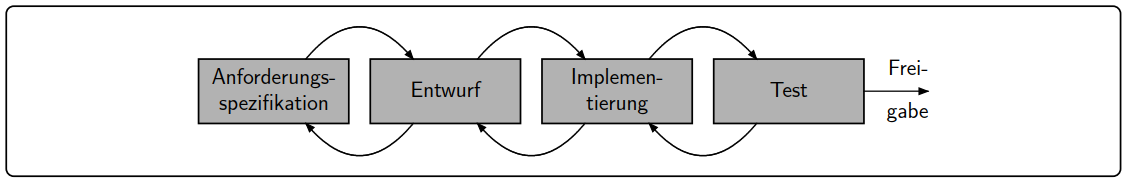
\includegraphics[width=14cm]{img/iterativesModell.png}
	\captionsetup{format=hang}
	\centering\caption[Iteratives Modell]{\label{fig:iteratModell}Iteratives Modell \\Quelle: Skript Systemanalyse S.25, Gregor Tielsch}
\end{figure}

Die zuvor vorgestellten Bestandteile sind aus dem Wasserfallmodell abgeleitet. Der Unterschied der beiden Modelle besteht in der Abarbeitung der verschiedenen Phasen. Während in dem Vorgängermodell, dem Wasserfallmodell, jede Phase der Reihe nach durchlaufen wird, sind in dem iterativen Modell Rücksprünge in vorige Phasen möglich. Dadurch lassen sich während der Entwicklung auftretende Änderungen und neue Anforderungen noch in das Softwareprodukt einarbeiten. Somit können die Entwicklungsfortschritte dem Kunden vorgestellt und sein Feedback eingearbeitet werden. 

\subsubsection{Anwendung des Teams}
Das Projektteam hat für die zu entwickelnde Software zunächst aus den Projektvorgaben von Hr. Tielsch die Anforderungen herausgezogen und mit einer Analyse zu bereits bestehenden Lösungen eines Kinoreservierungssystems begonnen. Mithilfe von Personas und User-Story-Mapping wurden typische Endnutzer modelliert, die die fertige Software nutzen werden. Außerdem wurde in der Entwurfsphase überlegt, wie die festgestellten Anforderungen umgesetzt werden können. Zusätzlich wurde mit dem Entwurf eines Prototyps angefangen. 

Die bis dahin erfolgten Ergebnisse wurden dem Kunden präsentiert und Feedback eingeholt. Nachfolgend hat das Team mit der Implementierung des Produkts begonnen. Gleichzeitig erfolgte ein Rücksprung in die erste Phase, um das Feedback des Kunden einarbeiten zu können. Dieses hat das Team außerdem dazu veranlasst eine erneute Ist-Analyse durchzuführen. Deren Ergebnisse wurden von dem Team umgesetzt, wodurch einzelne Produkte des Analysephase angepasst wurden. 

Nach dem Start aber vor Fertigstellung der Implementierung wurden bereits erste Tests geschrieben um die Funktionalität der bis dahin erstellten Software sicherzustellen. Durch das Weiterentwickeln der Software und dem gleichzeitigen Schreiben von Tests erfolgt ein ständiger Wechsel zwischen den Phasen Implementierung und Test. Dies liegt vor allem an der Teamgröße, da voneinander unabhängige Entwicklungen von den vielen Mitgliedern gleichzeitig erfolgen können. 
 
\section[Scrum]{Scrum{\hfill \normalsize Yvonne Werner}} \label{chapter:SCRUM}
Als Modell der Zusammenarbeit wurde Scrum gewählt, da dieses das gleichzeitige Arbeiten an verschiedenen Phasen des iterativen Modells erlaubt und fördert. Außerdem hat Scrum das Ziel ein agiles Umfeld für die Entwicklung und Auslieferung von Softwareprodukten zu schaffen. Da das iterative Modell ebenfalls eine agile Vorgehensweise darstellt, passen die gewählte Methode der Softwareentwicklung mit der Zusammenarbeit des Teams zusammen. 

\subsubsection{Theorie}
In Scrum steht vor allem die Interaktion innerhalb des Teams sowie zu Projektbetroffenen im Vordergrund. Außerdem wird versucht innerhalb von kurzen Zeitabständen funktionierende Software ausliefern zu können und durch die Agilität des Prozesses schnell auf Änderungen reagieren zu können. 

Zu Beginn eines Projekts werden alle bestehenden Anforderungen in dem Produkt Backlog festgehalten. Wie in Abbildung \vref{fig:scrum} ersichtlich ist, wird der Entwicklungsprozess für ein Produkt in kleinere Abschnitte, sogenannte Sprints, unterteilt. Die Sprint Planung, welche zu Beginn eines jeden Sprints stattfindet, dient der Auswahl von einzelnen Anforderungen, um welche das Produkt in dem nächsten Sprint erweitert werden soll. Zum Festhalten und Spezifizieren der gewählten Anforderungen dient der Sprint Backlog. Am Ende jedes Sprints ist das Ziel lauffähige Software vorweisen zu können. 

In einem Sprint kann sich dann jedes Teammitglied eine Teilaufgabe einer Anforderung heraussuchen, die es bearbeiten möchte. Das Entwicklungsteam arbeitet demnach selbstorganisiert und agil. Täglich findet ein kurzes Meeting statt, welches zum Ziel hat die anderen Mitglieder des Teams über den Fortschritt des letzten Tages, die nächsten Arbeitsschritte sowie Probleme zu informieren. Dadurch wird die Kommunikation des Teams gefördert und Probleme schnell aufgezeigt. Diese können nach dem Daily Scrum Meeting besprochen werden. 

\begin{figure}[H]
	\centering 
	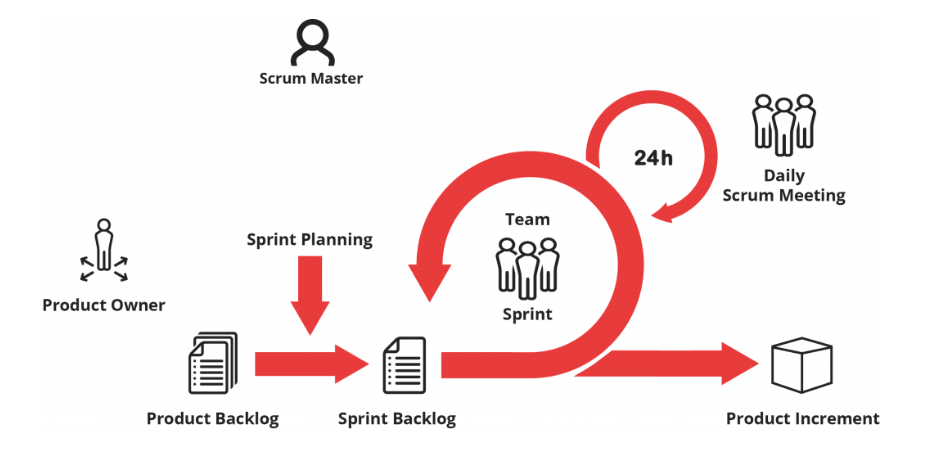
\includegraphics[width=14cm]{img/Scrum.png}
	\captionsetup{format=hang}
	\centering\caption[Iteratives Modell]{\label{fig:scrum}SCRUM \footnotemark}
\end{figure}
\footnotetext{https://www.etventure.de/blog/digitallearning-2-agiles-arbeiten-mit-scrum/}

Neben dem Team, welches die Entwicklung vornimmt, existieren weitere wichtige Rollen in Scrum. Der Product Owner ist für das Produkt verantwortlich und entscheidet durch Kundenkontakt, welche Funktionalitäten das Produkt erhalten soll und in welcher Reihenfolge. Der Scrum Master achtet darauf, dass die Regeln für Scrum eingehalten werden und hält Probleme von dem Team fern, damit es sich auf die Weiterentwicklung konzentrieren kann.  

\subsubsection{Umsetzung durch Team}
Die Rolle des Scrum Masters hat Fabio Westphal übernommen. Er hat mit dem Management des Teams auf regelmäßigen Kontakt des gesamten Teams geachtet. Außerdem hat er bei Fragen sich darum bemüht diese zeitnah zu klären. Die Rolle des Kunden hat Gregor Tielsch dargestellt, welcher die Projektdefinition sowie die Anforderungen gestellt hat. Dadurch hat er ebenfalls Teile des Product Owners übernommen, da er den Rahmen des Projekts eingeschränkt hat. Allerdings wurde von dem Team besprochen, welche Funktionalitäten zuerst in das Produkt eingebaut werden sollen. Außerdem sind durch die Bewertung und Gemeinschaftsarbeit des Projekts alle Projektbeteiligten für das Produkt verantwortlich. Deshalb kann die Rolle des Product Owners keiner Person eindeutig zugeordnet werden.

Die Länge eines Sprints betrug, wie auch in Abbildung \vref{fig:projektplan} ersichtlich ist, ungefähr drei Wochen. Aufgrund von anderen Lehrveranstaltungen fand keine tägliche Zusammenarbeit für das Projekt statt, weshalb die Notwendigkeit von täglichen Meetings nicht bestand. Um dennoch einen kontinuierlichen Austausch ermöglichen zu können, wurde Slack als Kommunikationsmittel verwendet. Alternativ zu einem Daily Scrum Meeting wurde ein Jour Fixe eingeführt, damit sich das Team in regelmäßigen Abständen (einmal wöchentlich) über den aktuellen Stand des Produkts informieren kann. 

Die Entwicklung durch das Team wurde teilweise mittels Pair-Programming durchgeführt. Dieses bildet eine agile Methode zur Entwicklung, bei der zwei gleichberechtigte Entwickler an einem Computer arbeiten. Dabei schreibt ein Entwickler den Code, während ein zweiter diesen auf Korrektheit überprüft. Beide Entwickler sind gleichberechtigt, was dazu führt, dass in regelmäßigen Abständen die Rollen getauscht werden.